% !TEX root = ../../Tesi_Triennale_PMNS.tex
\chapter[cWB]{Coherent WaveBurst: algoritmo per la rivelazione e la ricostruzione di segnali di onde gravitazionali}
\label{chapter:cwb}
La post coalescenza, come già detto, è allo stato attuale difficile da rivelare a causa della scarsa sensibilità dei detector a tali frequenze, per questo le analisi che vengono fatte in questa tesi non coivolgeranno dati misurati, ma dati simulati che vengono iniettati in rumore gaussiano, anch'esso simulato.

I dati che vengono forniti dal network di interferometri sono nella forma 
\[
x(t) = \xi_k(t) + n(t)
\]
dove $\xi_k$ è la risposta del detector dovuta all'effettiva onda gravitazionale, mentre n(t) è la serie di dati relativa al rumore.
Le risposte all'onda gravitazione del network sono scritte come
\begin{equation}
\xi_k[i,j] = F_{+,k}h_+[i,j] + F_{\times,k}h_\times[i,j]
\label{eqn:detector_response}
\end{equation}
dove $F_{+,k}(\theta,\phi)$ e $F_{\times,k}(\theta,\phi)$ sono gli antenna pattern del detector k-esimo\cite{Klimenko_2008}. In particolare gli antenna pattern descrivono la risposta del detector al passaggio dell'onda gravitazionale e dipendono dalla posizione della sorgente nel cielo e dall'angolo di polarizzazione. 

Per semplicità si introduce la seguente notazione:
\[
\mathbf{x}[i,j] = \left(x_1[i,j],\dots, x_K[i,j] \right) ;
\quad
%\mathbf{w}[i,j] = \left(\frac{x_1[i,j]}{\sigma_1[i,j]},\dots, \frac{x_K[i,j]}{\sigma_K[i,j]} \right) ;
\]
\[
\mathbf{h}[i,j] = (h_+[i,j], h_\times[i,j])
\quad
\mathbf{f}_{+(\times)}[i,j] = \left(\frac{F_{1+(\times)}[i,j]}{\sigma_1[i,j]},\dots, \frac{F_{K+(\times)}[i,j]}{\sigma_K[i,j]} \right) 
\]
dove K è il numero di detector nel network, $x_k[i,j]$ è il campione di dati del detector (l'indice i itera sui tempi, mentre l'indice j itera sulle frequenze)\cite{Klimenko_2008}, $h_{+}[i,j]$ e $h_{\times}[i,j]$ sono le ampiezze delle due polarizzazioni della GW e, mentre con la notazione $\sum_{\Omega_{TF}} = \sum_{i,j=1}^N$, in quanto si scriverà $\Omega_{TF}$ come il dominio tempo-frequenza.

%Con le notazioni precedenti e denotando il rumore $\mathbf{n}[i,j]$, si può scrivere
%\begin{equation}
%\mathbf{x}[i,j] = \mathcal{F}\mathbf{h}[i,j] + \mathbf{n}[i]
%\end{equation}
%con $\mathcal{F}$ la matrice di antenna pattern, definita come
%%\begin{wrapfigure}{r}{0.46\textwidth}
%%	\vspace{-10pt}
%%	\begin{center}
%%		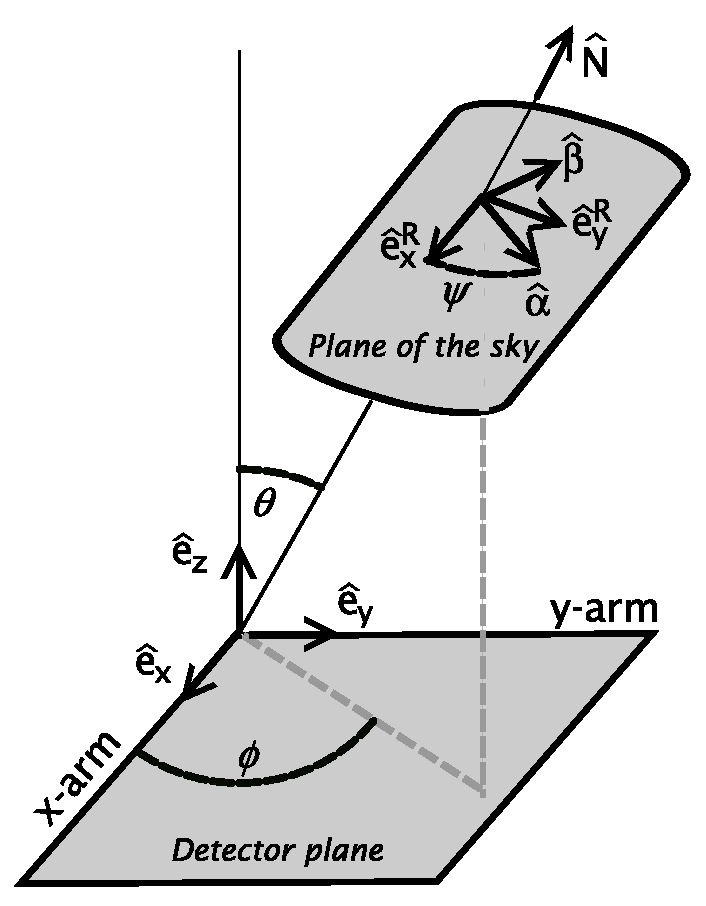
\includegraphics[width=0.25\textwidth]{figures/Capitolo_3/Detector_sky_full.eps}
%%	\end{center}
%%	\vspace{-5pt}
%%	\caption{L'orientazione relativa del piano delle polarizzazioni della GW e del piano su cui giacciono i bracci del detector, presa da \cite{Sathyaprakash_2009}.}
%%	\label{fig:antenna_pattern}
%%	\vspace{-30pt}
%%\end{wrapfigure}
%\begin{equation}
%\mathcal{F} = \begin{bmatrix}
%F_{1+}(\theta,\phi)	&F_{1\times}(\theta,\phi)\\
%\vdots					&   \vdots				 \\
%F_{K+}(\theta,\phi)	&F_{K\times}(\theta,\phi)\\
%\end{bmatrix}
%\end{equation}

%Gli antenna pattern descrivono come il detector riceve l'energia in funzione della posizione angolare e, in particolare, sono caratterizzati da una trasformazione basata sull'angolo di polarizzazione $\Psi$, equivalente alla rotazione del piano sul quale è definito $\mathbf{h}$.

%Nei metodi coerenti le statistiche vengono calcolate come somma coerente delle risposte dei detector singoli. Gli algoritmi che sfruttano questi metodi risultano più efficienti, devono cioè avere una probabilità di falso allarme più bassa, rispetto alle statistiche calcolate sulle risposte di ogni detector singolarmente.

L'algoritmo che si utilizza, Coherent WaveBurst (cWB), ricerca eccessi di potenza nella rappresentazione in un piano tempo-frequenza del segnale, coerenti fra i detector e quindi, attraverso l'utilizzo di una statistica coerente costituita da una analisi della massima verosimiglianza, combinando i dati dell'intero network, individua il pattern del segnale.\\
L'algoritmo differisce dai metodi tradizionali che identificano gli eventi nei detector singolarmente usando statistiche di eccesso di potenza e poi verificano la coerenza tra i segnali nei vari detector.
I vantaggi di questo tipo di analisi sono molteplici: innanzitutto la sensibilità del metodo non sarà limitata dal detector meno sensibile nel network, in quanto la likelihood utilizzata nei metodi coerenti rappresenta il rapporto segnale su rumore (SNR) totale del segnale ricostruito/rivelato dal network. 
Inoltre questo metodo permette di costruire altre statistiche coerenti, come il null stream o il coefficiente di correlazione  del network, per distinguere segnali che effettivamente hanno una controparte fisica rispetto a eccessi di rumore ambientale o strumentale. Infine, è possibile ricostruire la posizione celeste della sorgente\cite{Klimenko_2008}.

L'algoritmo cWB viene utilizzato all'interno della collaborazione LIGO-Virgo sia per l'analisi dei segnali in bassa latenza, per identificare e ricostruire candidati significativi e poter, una volta ottenuta una prima stima della posizione celeste della sorgente, condividerla con i telescopi partner per identificare i segnali elettromagnetici legati; sia per l'analisi di dati consolidati, volta a ottenere risultati più approfonditi sull'evento, stabilendo la significanza degli eventi osservati e identificando le stelle progenitrici\cite{Klimenko_2016}.
\section{Analisi coerente}
\label{section:coherent_analysis}
La pipeline di cWB per rivelare e ricostruire segnali utilizza un metodo basato sul rapporto di verosimiglianza, definito come il logaritmo del rapporto di verosimiglianza
\begin{equation}
	\Lambda(\mathbf{x},\Omega) = \frac{p(\mathbf{x}|\mathbf{h}(\Omega))}{p(\mathbf{x}|0)}
\end{equation}
dove $\Omega$ è il set di parametri che descrive il segnale, $p(\mathbf{x}|0)$ è la probabilità dell'ipotesi nulla, quindi di solo rumore strumentale, mentre $p(\mathbf{x}|\mathbf{h})$ è la probabilità composta che vi sia un segnale $\mathbf{h}$ nel campione $\mathbf{x}$\cite{Klimenko_2016}.


Nell'ipotesi idealistica di rumore gaussiano quasi stazionario, il funzionale può essere scritto in un piano tempo-frequenza come
\begin{equation}
	\mathcal{L} = \sum_{k=1}^{K}\sum_{i,j=1}^{N}\left(\frac{x_k^2[i,j]}{\sigma_k^2[i,j]} - \frac{(x_k[i,j]-\xi_k[i,j])^2}{\sigma_k^2[i,j]}  \right)
	\label{eqn:Likelihood}
\end{equation}
Il rumore del detector è caratterizzato dalla deviazione standard $\sigma_k[i,j]$,  anch'essa una funzione sul piano tempo-frequenza. I valori $w_k[i,j] = x_k[i,j]/\sigma_k[i,j]$ saranno i dati scalati con il rumore (detti sbiancati)\cite{Klimenko_2016}.



Dunque, al variare di $h_{+}[i,j]$ e $h_{\times}[i,j]$ varia anche $\mathcal{L}$, l'obiettivo è quindi ottenere i valori delle ampiezze che massimizzano il funzionale di verosimiglianza da cui si deduce la forma d'onda nel dominio dei tempi facendo una trasformazione di wavelet inversa.%, che consisterà dunque 

Il funzionale rapporto di verosimiglianza in equazione \ref{eqn:Likelihood} si può scrivere come
\begin{equation}
%	\mathcal{L} = \braket{w}{\xi} - \frac{1}{2} \braket{\xi}{\xi} = \mathcal{L}_+ + \mathcal{L}_\times = \sum_{\Omega_{TF}}\left[ \mathbf{w} \cdot \mathbf{f}_+ - \frac{1}{2}|\mathbf{f}_+|^2h_+^2\right] + \sum_{\Omega_{TF}}\left[ \mathbf{w} \cdot \mathbf{f}_\times - \frac{1}{2}|\mathbf{f}_\times|^2h_\times^2\right]
	\mathcal{L} =  \mathcal{L}_+ + \mathcal{L}_\times = \sum_{\Omega_{TF}}\left[ \mathbf{w} \cdot \mathbf{f}_+ - \frac{1}{2}|\mathbf{f}_+|^2h_+^2\right] + \sum_{\Omega_{TF}}\left[ \mathbf{w} \cdot \mathbf{f}_\times - \frac{1}{2}|\mathbf{f}_\times|^2h_\times^2\right]
	\label{eqn:label_separated}
\end{equation}
dove i vettori di antenna pattern $\mathbf{f}_+$ e $\mathbf{f}_\times$ sono definiti nel Dominant Polarisation wave Frame (DPF), ovvero il piano in cui entrambi gli antenna pattern sono reali, definiti positivi e vale $\mathbf{f}_+ \cdot \mathbf{f}_\times = 0$.  Alla luce di questo, per ottenere la massima verosimiglianza si dovrà risolvere le equazioni:
\begin{equation}
%	\mathbf{w} \cdot \mathbf{f}_+ = |\mathbf{f}_+|^2h_+ \quad\quad\quad  \mathbf{w} \cdot \mathbf{f}_\times = |\mathbf{f}_+|^2h_\times 
	\begin{bmatrix}
	(\mathbf{w}[i,j]\cdot \mathbf{e}_+[i,j])\\
	(\mathbf{w}[i,j]\cdot \mathbf{e}_\times[i,j])
	\end{bmatrix}
	=
	\begin{bmatrix}
	\mathbf{f}_+[i,j]	&0\\
	0					&\mathbf{f}_\times[i,j]
	\end{bmatrix}
	\begin{bmatrix}
	h_+[i,j]\\
	h_\times[i,j]\\
	\end{bmatrix}
	\label{eqn:sistema_soluzione}
\end{equation}
%La massima verosimiglianza può essere scritta quindi sostituendo le soluzioni di \ref{eqn:sistema_soluzione} in $\mathcal{L}(h)$, che restituisce
%\begin{equation}
%	L_{max} = \sum_{\Omega_{TF}}\mathbf{w}[i,j]P[i,j]\mathbf{w}^\intercal[i,j]
%\end{equation}
%dove la matrice $P$ è il proiettore costruito a partire dai versori $\mathbf{e}_+$ e $\mathbf{e}_\times$:
%\begin{equation}
%	P_{nm}[i,j]=e_{n+}[i,j]e_{m+}[i,j]+e_{n\times}[i,j]e_{m\times}[i,j]
%	\label{eqn:proiection}
%\end{equation}

%\paragraph{Regolatori} C'è una particolare classe di vincoli, i regolatori, che dipendono da come il network reagisce a un determinato segnale. Si può citare un esempio considerando il caso in cui $|f_\times|=0$, come nel caso di detector allineati; la risposta del network dovrebbe essere lungo la direzione di $f_+$ e imporre questo vincolo porta l'analisi della likelihood a ignorare la risposta-$\times$ del network. Anche per detector non allineati si utilizzano questo tipo di vincoli: in base alla posizione della sorgente, il network può essere meno sensibile alla seconda componente della GW ($|\mathbf{f}_\times|^2 \ll |\mathbf{f}_+|^2$) portando a problemi nella ricostruzione di $h_\times$. Quello che viene fatto da cWB è cambiare la norma di $\mathbf{f}_\times$ con un parametro $\delta$, equivalente ad aggiungere un ulteriore detector al network che permette di preservare l'ortogonalità di $\mathbf{e}_+ \text{ e } \mathbf{e}_\times'$.
\section{Algoritmi per l'analisi dati}
L'algoritmo, scritto in C++/ROOT e sviluppato da LIGO Scientific Collaboration, può lavorare senza nessuna assunzione a priori sulla forma del segnale o sulla sorgente, come viene utilizzato in questa tesi, o con assunzioni deboli sul modello del segnale.\\
Vengono descritti i principali step dell'algoritmo: trasformazione di wavelet, generazione di trigger coerenti e selezione dei trigger coerenti.
\subsection{Trasformazioni di wavelet}
\label{subsection:wavelet_transform}
Le trasformazioni di wavelet, partendo dai dati discreti, producono rappresentazioni tempo-frequenza dei dati dei rivelatori $w[i,j]$. Lo spettro di wavelet può essere quindi rappresentato con uno scalogramma tempo-frequenza. La risoluzione nel dominio del tempo $\Delta t_j(R)$ è determinata dal rate di campionamento R e dall'indice di scala j. Poiché le trasformazioni di wavelet costituiscono una serie di trasformazioni di Fourier infinitesime, conservano il volume del campione, pari a 1/2 per la serie temporale in input.

\begin{wrapfigure}{r}{0.46\textwidth}
	\vspace{-15pt}
	\begin{center}
		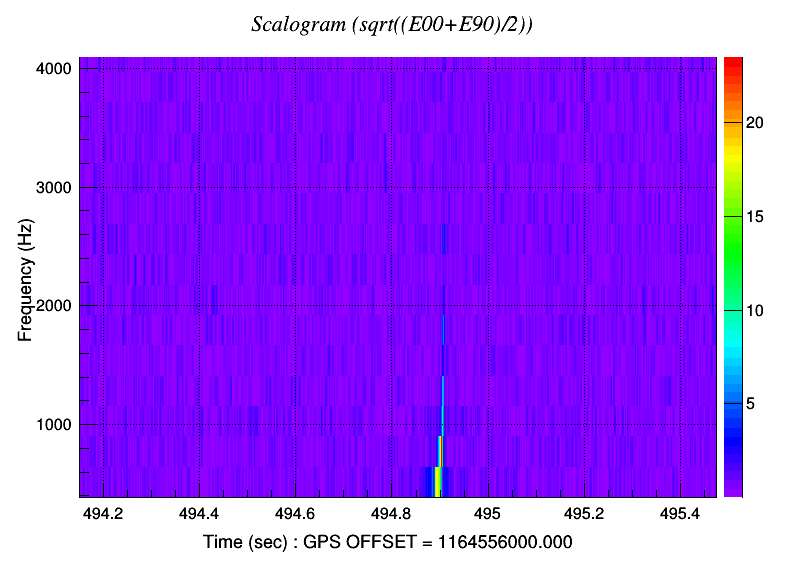
\includegraphics[width=0.475\textwidth]{figures/Capitolo_3/L1_scalogram_0.png}
	\end{center}
	\vspace{-5pt}
	\caption{Scalogramma ottenuto da una analisi di una simulazione di coalescenza di una BNS con EOS SHT2.0 con rumore gaussiano del detector LIGO Hanford}
	\label{fig:scalogram_example}
	\vspace{-40pt}
\end{wrapfigure}
Si avrà quindi una risoluzione in frequenza $\Delta f_j$ definita come 1/(2$\Delta t_j$) che determina la larghezza di banda per l'indice j. Per ottimizzare la ricerca nel piano, cWB procede con diverse trasformazioni a risoluzioni diverse, che permette di ottenere il grafico in figura \ref{fig:scalogram_example}.
%\subsection{Filtro di predizione lineare dell'errore}
%\label{subsection:lpe_filter}
%I filtri per la predizione lineare dell'errore (LPE) sono usati per rimuovere le componenti prevedibili dalla serie temporale in input. Possono essere applicati nel dominio di wavelet, ma più frequentemente vengono usati nel dominio temporale restituendo una serie temporale sbiancata.
%
%Ogni layer di wavelet (quindi a frequenza fissata) è una serie temporale, perciò anzichè applicare il filtro LPE alla sere temporale $x(t)$, si può fare prima una decomposizione di wavelet $x(t)\rightarrow w(f,t)$ e quindi applicare il filtro ad ogni layer di wavelet. Si ottiene dunque un campione $w'(f, t)$ da cui è possibile ricostruire la serie temporale sbiancata $x'(t)$ attraverso una trasformazione di wavelet inversa\cite{Klimenko_2008}.
%\subsection{Filtri per il ritardo temporale nel dominio di wavelet}
%\label{subsection:time_delay_filters}
%Per la valutazione della likelihood è necessario computare il prodotto scalare $\bra{x_n(\tau_n)}\ket{x_m(\tau_m)}$, dove bisogna considerare un ritardo intrinseco del set di dati del rivelatore $n$ rispetto a $m$, in quanto le GW viaggiano a velocità finita pari a $c$. Dunque il ritardo temporale $\tau_n - \tau_m$ dipende dalla posizione $(\theta, \phi)$ della sorgente.
%
%Nel dominio di wavelet è invece necessario calcolare il prodotto interno $\bra{w_n(\tau_n)}\ket{w_m(\tau_m)}$, le ampiezze ritardate possono essere calcolate a partire dalle ampiezze originali utilizzando un filtro di ritardo temporale $D_{kl}(\tau)$
%\begin{equation}
%	w_{n,m}(i,j,\tau) = \sum_{kl}D_{kl}(\tau, j)w_{n,m}(i+k, j+l)
%	\label{eqn:time_filter}
%\end{equation}
%dove $k$ ed $l$ sono le coordinate locali nel piano tempo-frequenza rispetto alla posizione $(i,j)$.
%
%La costruzione di questi filtri è legata alla decomposizione delle funzioni di wavelet ritardate $\Psi_j(t+\tau)$ nella base delle funzioni non traslate $\Psi_j(t)$. Si procede dunque per step:
%\begin{enumerate}
%	\item viene creata una serie di wavelet con un solo coefficiente pari all'unità nella posizione $(i,j)$;
%	\item viene applicata la trasformazione di wavelet inversa ricostruendo $\Psi_j(t)$ nel dominio dei tempi;
%	\item viene applicata la traslazione temporale $\Psi_j(t)\rightarrow\Psi_j(t+\tau)$ e si decompone quest'ultima;
%	\item le ampiezze di wavelet ottenute nelle posizioni $(i+k, j+l)$ rappresentano i coefficienti del filtro $D_{kl}(\tau, j)$ per il layer j.
%\end{enumerate}
%L'applicazione di questo filtro porta a una perdita di energia, valutabile in $\epsilon_K = 1 - \sum_{K}D_{kl}^2$
%%\begin{equation}
%%	\epsilon_K = 1 - \sum_{K}D_{kl}^2
%%	\label{eqn:energy_loss}
%%\end{equation}
%e perciò la lunghezza del filtro sarà legata alla quantità di energia acsecettabile da perdere (valori tipici sono $K>20$ per ottenere una perdita di energia inferiore a $1\%$)\cite{Klimenko_2008}.
\subsection{Generazione di trigger coerenti}
\label{section:coherent_trigger}
La generazione dei trigger, quindi l'identificazione dei segnali, è basata su statistiche di eccesso di potenza e di correlazione incrociata tra i segnali dei detector. 

Il funzionale di likelihood viene calcolato come somma sui campioni selezionati per l'analisi, il numero di termini sommati dipende all'area nel piano tempo-frequenza che si considera, se tale somma consiste di un solo elemento si può scrivere il funzionale come
\begin{equation}
	\mathcal{L}_p(i,j,\theta,\phi)=|\mathbf{w}|^2 -|\mathbf{w} - \mathbf{f}_+h_+ - \mathbf{f}_\times h_\times|^2
	\label{eqn:likelihood_single_term}
\end{equation}

\begin{wrapfigure}{r}{0.46\textwidth}
	\vspace{-25pt}
	\begin{center}
		\includegraphics[width=0.475\textwidth]{figures/Capitolo_3/l_tfmap_scalogram.png}
	\end{center}
	\vspace{-5pt}
	\caption{Mappa di Likelihood ottenuta da una analisi di una simulazione di coalescenza di una BNS con EOS SHT2.0 con rumore gaussiano del network LIGO-Virgo}
	\label{fig:Likelihood_example}
	\vspace{-10pt}
\end{wrapfigure}
Poiché è possibile applicare il metodo della likelihood al funzionale \ref{eqn:likelihood_single_term}, si può trovare il massimo $L_p(\theta, \phi)$ al variare di $h_+$ e $h_\times$ e quindi ricercare il massimo in funzione della posizione celeste
\begin{equation}
	L_m(i,j)= \max_{\theta, \phi}[L_p(i,j,\theta,\phi)]
	\label{eqn:max_L}
\end{equation}
La statistica $L_m$ ha quindi il significato della massima energia rivelata dal network in una determinata posizione del piano tempo-frequenza. Selezionando quindi i valori di $L_m$ sopra una determinata soglia si può identificare un cluster di pixel come potenziale segnale di GW. In questo modo si identificano i segnali combinando i dati dell'intero network e non si cercano i segnali sui singoli detector, verificando successivamente la coerenza.
A questo punto si devono ricostruire i parametri del segnale legato al trigger, incluse la posizione della sorgente, le due polarizzazioni della GW, le risposte individuali dei rivelatori e le statistiche di massima likelihood dei trigger. In particolare la likelihood è ricostruita come
\begin{equation}
	\mathcal{L}_c(\theta,\phi) = \sum_{i,j}\mathcal{L}_p(i,j,\theta, \phi)
\end{equation}
La massima likelihood $L_{max}$ è ottenuta facendo variare $\mathcal{L}_c$ su $\theta$ e $\phi$ ed è calcolata su tutti i pixel di likelihood nel piano tempo frequenza per formare il trigger coerente\cite{Klimenko_2008}.
\subsection{Selezione dei trigger coerenti}
Nel caso di rumore gaussiano stazionario la massima verosimiglianza è l'unica statistica necessaria per la rivelazione e per la selezione degli eventi, per cui la probabilità di falso allarme e di scartare eventi effettivi è legata alla soglia minima per $L_{max}$. Nella realtà tuttavia il rumore non è tale, ma i dati sono sporcati da rumore strumentale e ambientale, per cui è necessario applicare altri metodi per distinguere i segnali reali. Alcuni esempi, utilizzati da cWB sono le statistiche coerenti ricavate dalle matrici di verosimiglianza e null.
La matrice di likelihood $L_{mn}$ è ottenuta dalla forma quadratica della likelihood
%da completare la parte dei regolatori a cui questa parte fa riferimento.
\begin{equation}
	L_{max} = \sum_{mn}L_{mn} = \sum_{mn}\left[\left< w_nw_me_{+n}e_{+m} \right> + \left< w_nw_me_{\times n}e_{\times m} \right>\right]
	\label{eqn:likelihood_matrix}
\end{equation}
dove $m\text{ e }n$ sono gli indici che identificano i detector\cite{Klimenko_2008}. Gli elementi della diagonale di $L_{mn}$ descrivono l'energia incoerente normalizzata, mentre quelli dell'antidiagonale sono espressione dell'energia coerente normalizzata, la cui somma restituisce l'energia coerente totale $E_{coh}$ rivelata dal network
\begin{equation}
	E_{inc} = \sum_{\Omega_{TF}}\sum_{n}w_n[i,j]P_{mn}[i,j]w_n[i,j],
	\quad\quad
	E_{coh} = \sum_{\Omega_{TF}}\sum_{m\neq n}w_n[i,j]P_{mn}[i,j]w_n[i,j].
\end{equation}
dove la matrice $P$ è il proiettore costruito a partire dai versori $\mathbf{e}_+$ e $\mathbf{e}_\times$: $P_{nm}[i,j]=e_{n+}[i,j]e_{m+}[i,j]+e_{n\times}[i,j]e_{m\times}[i,j]$. 
Queste statistiche coerenti sono particolarmente utilizzate per la ricerca di segnali e la ricostruzione\cite{Klimenko_2016}.
Si può dunque esprimere i coefficienti di correlazione per detector allineati e quindi l'energia coerente ridotta
\begin{equation}
	r_{mn} = \frac{L_{mn}}{\sqrt{L_{nn}L_{mm}}} \quad\quad\quad \rightarrow \quad\quad\quad e_{coh}=\sum_{ n\neq m}L_{nm}|r_{nm}|
	\label{eqn:coherent_energy}
\end{equation}
quest'ultima in particolare risulta uno dei parametri più efficienti per l'accettazione/rifiuto di un trigger.

La matrice di null rappresenta l'energia normalizzata del rumore ricostruito
\begin{equation}
	N_{nm} = E_{nm}-L_{nm}
\end{equation}
con $E_{mn}$  è la matrice diagonale delle energie normalizzate dei detector $E_{mm}  = \left<x_m^2\right>$. Per distinguere i segnali effettivi da rumore strumentale e ambientale si usano i coefficienti di correlazione 
\begin{equation}
	C_{net} = \frac{E_{coh}}{N_{ull}+|E_{coh}|}, \quad\quad\quad c_{net} = \frac{e_{coh}}{N_{ull}+|e_{coh}|}
	\label{eqn:coefficient_energy}
\end{equation}
dove $N_{ull}$ è la somma di tutti gli elementi della matrice null, che rappresenta l'energia totale nella serie null. Accade infatti che eccessi di rumore vengano ricostruiti come segnale: i coefficienti $C_{net}$ e $c_{net}$ sono usati quindi come verifica della consistenza del segnale in quanto comparano l'energia del null e l'energia coerente\cite{Klimenko_2008},in particolare un evento genuino risulta per $c\smallsim 1$, mentre per $c \ll 1$ corrisponde ad un evento spurio\cite{Klimenko_2016}.

%Introduzione sull'algoritmo fatta nel paragrafo precedente, magari riprenderla veltocemente.
%Coherent analysis, significato e descrizione della likelihood: spiega quindi bene la differenza con gli algoritmi classici di confronto con segnali già modellati.

%regolatori, antenna pattern 

%algoritmi utilizzati: wavelet transformation, (linear predicion error), mappa verosimiglianza, mappa energia coerente (con piccoli grafici esemplificativi)

%(cenni sulla trasformazione di fase)


%\lipsum[3]\cite{Abbott_2017a}.
%
%\lipsum[4]\cite{Klimenko_2008}.
%
%\lipsum[6]\cite{Klimenko_2016}.
%
%\section{Esempi di analisi utilizzando cWB}
%\label{section:examples}
%Vengono ora riportati alcuni esempi di analisi di eventi simulati utilizzando cWB, partendo da forme d'onda simulate a partire da due diverse EOS. 
%%In particolare per ogni analisi verranno riportati i seguenti grafici e coefficienti:
%%\begin{itemize}
%%		\item il 
%%		\item i grafici dell'ampiezza di strain ricostruita nel dominio dei tempi e nel dominio delle frequenze relative a un solo rivelatore.		
%%\end{itemize}
%\subsection{Equazione di stato APR4}
%\label{subsection:APR4}
%\begin{minipage}[c]{0.55\textwidth}
%	Si riportano i principali coefficienti per identificare l'evento: il rapporto segnale su rumore (SNR); il valore del coefficiente $\rho$, ovvero una ranking statistic che esprime la significanza del segnale descrivendo l'ampiezza correlata effettiva; il coefficiente $c_{net}$ descritto in equazione \ref{eqn:coefficient_energy}; ED che descrive lo sbilanciamento dell'energia tra i detector nel network e, infine, $\theta$ e $\phi$ che descrivono la posizione celeste della sorgente;
%\end{minipage}
%\hspace{5mm}
%\begin{tabular}{cccccc}
%	\toprule
%	SNR	&$\rho$	&$c_{net}$	&ED	&$\theta$	&$\phi$	\\
%	\midrule
%	103.1	&50.8	&0.97	&-0.1	&101.6	&-28.6	\\
%	\bottomrule
%\end{tabular}
%\begin{figure}[H]
%	\vspace{-20pt}
%	\centering
%	\subfloat[][\emph{LIGO-Livingstone}]
%	{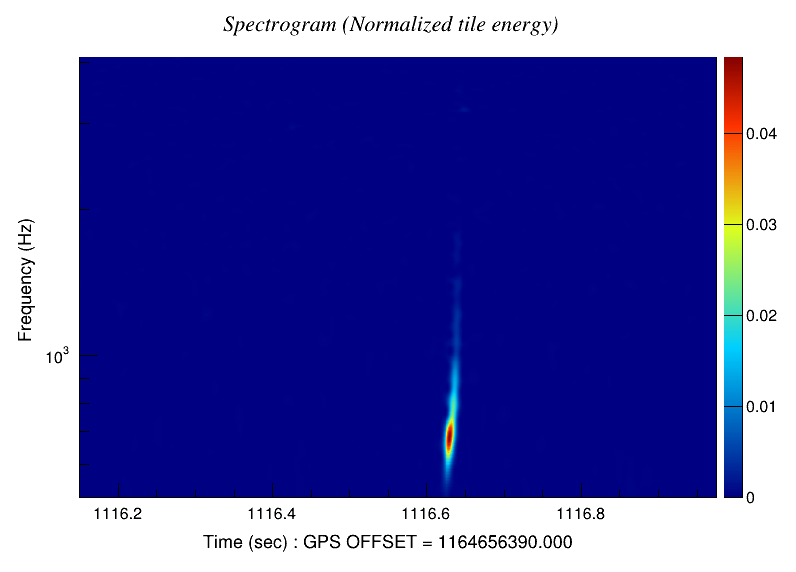
\includegraphics[width=.318125\textwidth]{figures/Capitolo_3/APR4_q09/L1_spectrogram_logy_0.png}} \quad
%	\subfloat[][\emph{LIGO-Hanford}]
%	{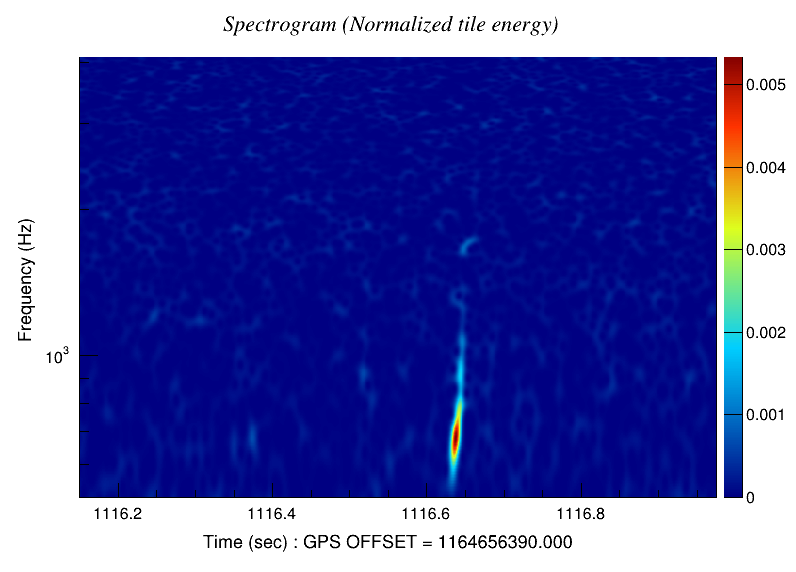
\includegraphics[width=.318125\textwidth]{figures/Capitolo_3/APR4_q09/H1_spectrogram_logy_0.png}} \quad
%	\subfloat[][\emph{Virgo}]
%	{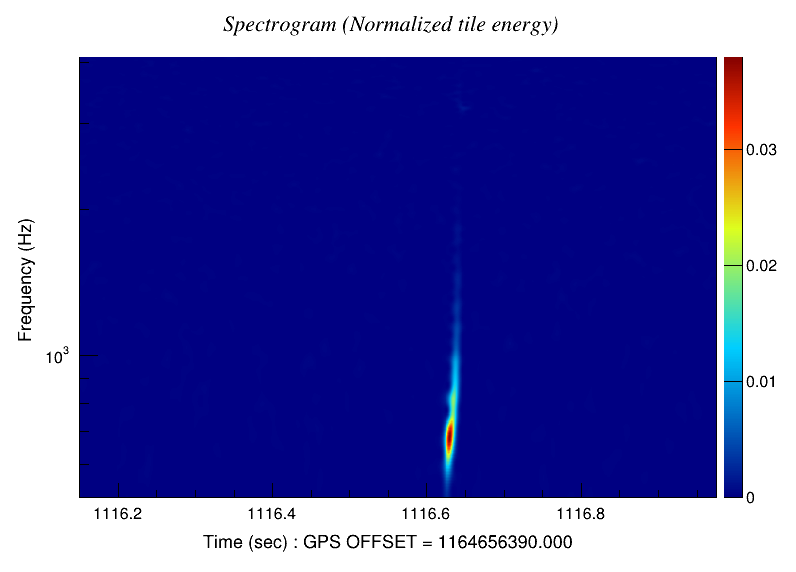
\includegraphics[width=.318125\textwidth]{figures/Capitolo_3/APR4_q09/V1_spectrogram_logy_0.png}}
%	\vspace{-5pt}
%	\caption{Spettrogrammi per ciascun detector, che mostrano una rappresentazione sul piano tempo-frequenza del trigger, basandosi sulla scomposizione di Fourier}
%	\label{fig:spettrogramma_apr4}
%	\vspace{-15pt}
%\end{figure}
%\begin{wrapfigure}{r}{0.46\textwidth}
%	\vspace{-10pt}
%	\begin{center}
%		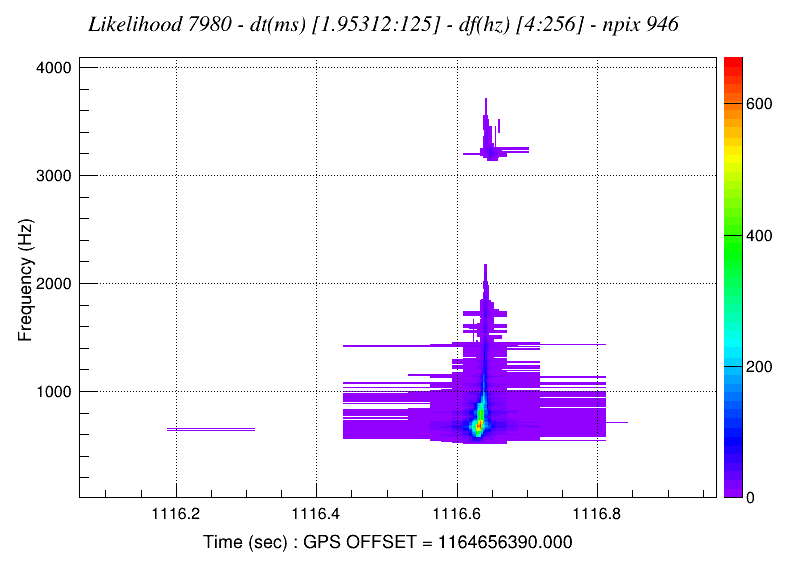
\includegraphics[width=0.475\textwidth]{figures/Capitolo_3/APR4_q09/l_tfmap_scalogram.png}
%	\end{center}
%	\vspace{-5pt}
%	\caption{Mappa di verosimiglianza nel piano tempo-frequenza, che descrive il contributo dell'energia totale del campione associato all'evento ricostruito}
%	\label{fig:Likelihood_APR4}
%	\vspace{-10pt}
%\end{wrapfigure}
%Il segnale che si mostra è particolarmente energetico, perché è stato simulato ad una distanza molto ravvicinata ($d \simeq 1.25$Mpc). Si osservano quindi coefficienti particolarmente elevati.
%Come si può osservare in Figura \ref{fig:spettrogramma_apr4}, mentre i detector LIGO-Livingstone e LIGO-Handford rivelano in modo evidente un segnale già ad un'analisi visiva, senza rumore significativo a sporcare la rivelazione, nella mappa di Virgo risulta distinguibile il segnale, tuttavia con rumore significativo e si può notare anche come guardando la scala di significanze del segnale questo risulti di un ordine di grandezza inferiore per Virgo, rispetto ai due rivelatori LIGO. Questo è probabilmente dovuto al fatto che i rivelatori LIGO sono allineati tra loro, mentre disallineati rispetto a Virgo e soprattutto alla posizione celeste della sorgente, favorevole ai primi due.
% 
%Nel grafico della likelihood in figura \ref{fig:Likelihood_APR4}, si osserva una tipica figura a chirp, in cui la parte inferiore, a basse frequenze, rappresenta l'inspiral fino alla coalescenza, mentre il cluster di dati in alto, a frequenze particolarmente elevate ($\smallsim 3.3$KHz) corrisponde all'emissione del post-merger.
%Infine nei grafici che seguono in figura \ref{fig:strain_apr4} si osservano le ricostruzioni della forma d'onda, in particolare in nero è plottato il segnale iniettato nella simulazione, mentre in rosso il segnale ricostruito. In particolare osservando il grafico delle frequenze si può notare come non sia stato ricostruito tra $\smallsim2.5$KHz e $\smallsim3$KHz, giustificando la separazione tra i cluster nel grafico della likelihood.
%\begin{figure}[H]
%	\vspace{-20pt}
%	\centering
%	\subfloat[][\emph{Dominio dei tempi}]
%	{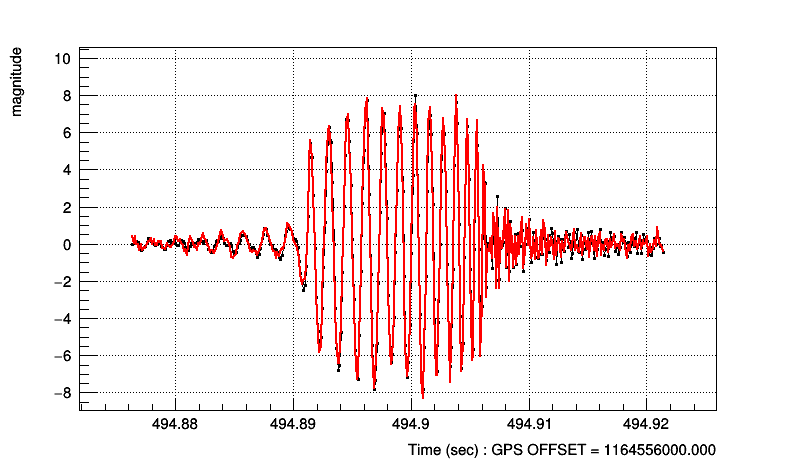
\includegraphics[width=.45\textwidth]{figures/Capitolo_3/APR4_q09/L1_wf_white_inj_rec.png}} \quad
%	\subfloat[][\emph{Dominio delle frequenze}]
%	{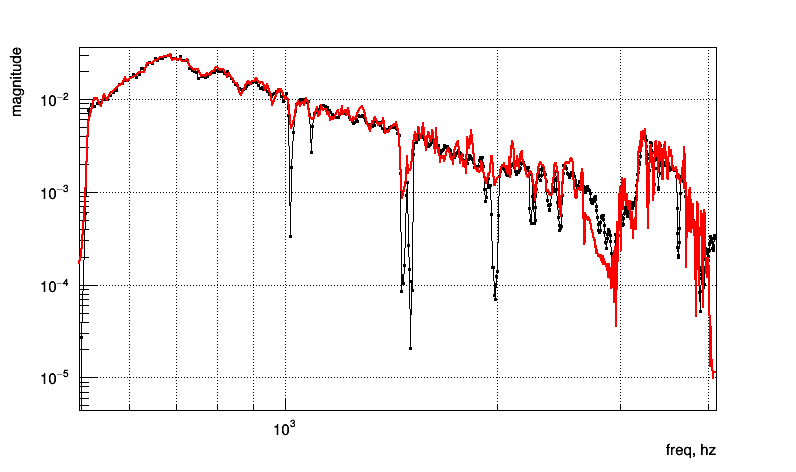
\includegraphics[width=.45\textwidth]{figures/Capitolo_3/APR4_q09/L1_wf_white_inj_rec_fft.png}}
%	\vspace{-5pt}
%	\caption{Ampiezza di strain ricostruita nel dominio dei tempi e nel dominio delle frequenze relative a un solo rivelatore}
%	\label{fig:strain_apr4}
%	\vspace{-15pt}
%\end{figure}
%\subsection{Equazione di stato SHT2}
%\label{subsection:SHT2}
%Per motivi di spazio non verranno presentate le analisi complete, come per l'equazione di stato precedente, ma si mostreranno solo i grafici delle likelihood: le due forme d'onda iniettate differiscono per la massa delle NS per la coalescenza, in particolare nella \ref{fig:likelihood_sht2}(a), con masse tali da andare in ipermassiva, si può notare come sia presente un segnale di post-merger a $\smallsim 2.5$kHz mentre nella \ref{fig:likelihood_sht2}(b), che ha masse tali da andare direttamente in buco nero, non vi è nessun segnale di post-merger ma solo un segnale di merger che arriva ad alte frequenze. 
%\begin{figure}[H]
%	\vspace{-20pt}
%	\centering
%	\subfloat[][\emph{SHT2.0}]
%	{\includegraphics[width=.4\textwidth]{figures/Capitolo_3/SHT2.0spinf1_1/l_tfmap_scalogram.png}} \quad
%	\subfloat[][\emph{SHT2.2}]
%	{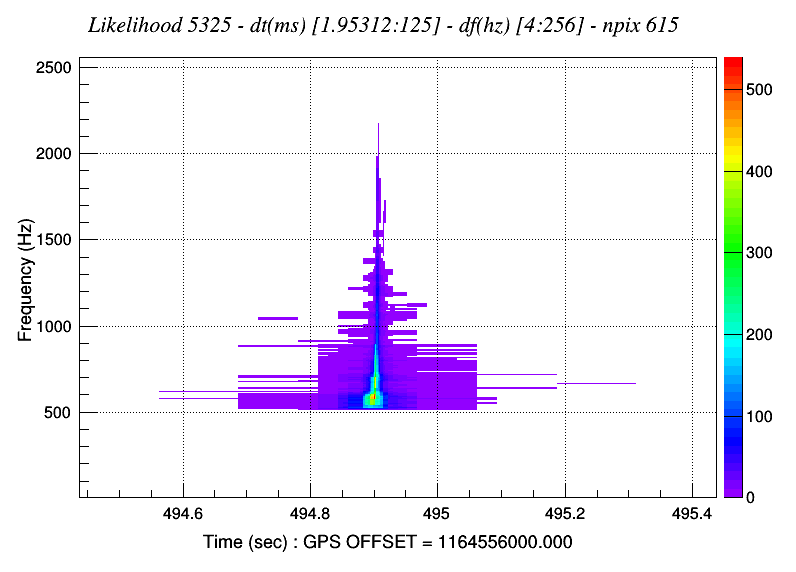
\includegraphics[width=.4\textwidth]{figures/Capitolo_3/SHT2.2spinf1_1/l_tfmap_scalogram.png}}
%	\vspace{-5pt}
%	\caption{Mappe di verosimiglianza ricostruite per le due forme d'onda iniettate}
%	\label{fig:likelihood_sht2}
%	\vspace{-15pt}
%\end{figure}